\chapter{Implementação da solução}
\label{cap:implementacao}

Neste capítulo apresenta-se a prova de conceito da solução proposta, demonstrando a viabilidade da arquitetura definida no capítulo anterior, seguida da implementação da mesma. Esta permite testar os principais componentes do sistema, as tecnologias utilizadas e o fluxo de comunicação que assegura a recolha, assinatura, validação e registo do consentimento digital. Por fim, são apresentados os resultados dos testes funcionais, que permitem avaliar se a implementação cumpre os objetivos definidos para o sistema.

\section{Prova de Conceito}

O objetivo é demonstrar a viabilidade técnica e conceptual da \textit{Prova de Consentimento} apresentada no Capítulo~\ref{cap:arquitectura}, validando os princípios de autenticidade, integridade, não repúdio, transparência e auditabilidade sem recorrer a uma implementação completa.

O registo de consentimento é representado como um objeto estruturado, contendo o \textit{payload} com as decisões do utilizador, a assinatura digital do próprio utilizador (gerida através da extensão) e a assinatura digital do servidor. Esta abordagem demonstra que o sistema suporta múltiplas assinaturas sobre o mesmo conteúdo, conforme previsto na \textit{JSON Serialization} do \textit{JWS}, assegurando verificabilidade e auditabilidade mesmo num modelo simplificado.

A prova de conceito permite confirmar que é possível gerar, assinar e verificar registos de consentimento de forma independente, validando a integridade e autenticidade dos dados e assegurando o não repúdio. Além disso, evidencia que a arquitetura conceptual é flexível e pode ser posteriormente implementada num protótipo funcional com componentes reais, incluindo extensões de navegador, servidores e CMPs diferentes. Assim, esta demonstração serve como validação experimental da arquitetura, reforçando a confiança na abordagem e evidenciando os benefícios do modelo proposto.

\section{Prova de conceito e testes funcionais}

O \textit{back-end} do servidor foi desenvolvido em \textit{Node.js}, enquanto o website é constituído por uma página em \textit{HTML} simples, integrando um \textit{snippet} do \textit{script} de um \acrshort{cmp} \textit{Open-Source} (\textit{klaro.js}) para a apresentação do \textit{banner} de consentimento.
Esta escolha oferece maior flexibilidade: permite que a solução seja utilizada como base para o desenvolvimento de sistemas próprios, sem a necessidade de criar um CMP do zero. Isto reduz o esforço de implementação e facilita a integração com diferentes navegadores, serviços ou fluxos de consentimento. Para o utilizador, o benefício reside não apenas na possibilidade de verificar e auditar o funcionamento da ferramenta, mas também na garantia de que os seus consentimentos são processados de forma consistente e que a implementação pode ser adaptada para reforçar a sua privacidade e controlo sobre os dados.
Do lado do cliente, foi implementada uma extensão de navegador em JavaScript, responsável pela captura das interações do utilizador e pela execução das operações criptográficas necessárias. Embora se trate de uma extensão em JavaScript nativo, recorreu-se ao \textit{Vue.js} como \textit{framework}, em conjunto com o Vite como \textit{bundler}, de modo a permitir a integração de bibliotecas externas, nomeadamente o \texttt{node-forge} para o tratamento de chaves e certificados. Adicionalmente, o processo de criação e gestão de certificados digitais foi realizado com recurso a o \textit{OpenSSL}. O fluxo de comunicação resultante contempla as etapas de recolha, assinatura, envio, validação e registo do consentimento em ambas as entidades, assegurando a autenticidade, integridade e verificabilidade do processo.

\subsection{JWS}

No âmbito da gestão do consentimento, a organização e validação dos mesmos exigem um formato seguro, interoperável e verificável. Entre várias alternativas, optou-se por utilizar o \textit{JSON Web Signature} (\textit{JWS}), conforme definido no RFC 7515 \citep{rfc7515}.

\subsubsection{Descrição Geral}

De acordo com o RFC 7515, um \textit{JWS} representa conteúdos protegidos com assinaturas digitais ou códigos de autenticação de mensagem (MAC) \citep{NISTMAC}, usando estruturas de dados em JSON.

Existem duas formas de serialização definidas:

\begin{itemize}
  \item \textit{Compact Serialization}: uma representação mais concisa, adequada a ambientes com restrições de espaço, como cabeçalhos HTTP ou parâmetros de URL.
  \item \textit{JSON Serialization}: uma representação em JSON que permite múltiplas assinaturas ou MACs sobre o mesmo conteúdo, com maior clareza e flexibilidade.
\end{itemize}

O \textit{JWS} baseia-se em três componentes principais:

\begin{enumerate}
  \item \textit{Header}: contém metadados como o algoritmo de assinatura (por exemplo, \texttt{PS256} \citep{Auth0SigningAlgorithms}), o tipo de objeto (por exemplo, \texttt{JWT}), e possivelmente outros parâmetros relevantes.
  \item \textit{Payload}: o conteúdo a assinar que é codificado em Base64URL.
  \item \textit{Signature}: o resultado da assinatura digital aplicada ao \textit{header} e \textit{payload}, garantindo integridade e autenticidade.
\end{enumerate}

\subsubsection{Aplicação ao Caso de Consentimento}

No sistema implementado, o consentimento do utilizador é representado através de um \textit{JWS}, com estas características específicas:

\begin{itemize}
  \item O \textit{payload} inclui informação relevante sobre o consentimento (por exemplo, serviços aceites/rejeitados).
  \item O \textit{header} utiliza o algoritmo \texttt{PS256}, que combina RSASSA-PSS com SHA-256, tendo sido escolhido devido às suas vantagens de segurança face ao RS256. O PS256 utiliza o esquema de preenchimento probabilístico (PSS), gerando assinaturas diferentes para o mesmo \textit{header} e \textit{payload}, o que aumenta a resistência contra ataques a assinaturas determinísticas e fornece maior robustez criptográfica \citep{ScottBrady2020}.
  \item São produzidas, pelo menos, duas assinaturas:
    \begin{itemize}
      \item Uma assinatura gerada pelo cliente (extensão do navegador), garantindo que foi o utilizador quem autorizou o consentimento.
      \item Outra assinatura adicional do servidor, garantindo que o servidor valida e “assina” o consentimento final, reforçando a confiabilidade e verificabilidade.
    \end{itemize}
\item A presença de múltiplas assinaturas segue o modelo da \textit{JSON Serialization} do \textit{JWS}, que suporta várias assinaturas sobre o mesmo \textit{payload}.
\end{itemize}

\subsubsection{Vantagens neste contexto}

Neste contexto, a utilização do \textit{JWS} oferece várias vantagens. Em primeiro lugar, garante a integridade e autenticidade do consentimento, uma vez que qualquer modificação no \textit{payload} ou nas assinaturas invalida o \textit{JWS}, protegendo contra manipulação. 
Em segundo lugar, assegura o não repúdio, uma vez que as assinaturas do cliente e do servidor permitem verificar se o consentimento foi efetivamente fornecido pelo utilizador e validado pelo servidor.
Além disso, tanto o cliente como o servidor conseguem verificar de forma independente a autenticidade do consentimento, reforçando a confiança no processo.
Por fim, o \textit{JWS} segue padrões abertos e é interoperável, o que facilita a integração com outras ferramentas e sistemas, permitindo que os registos de consentimento sejam utilizados de forma consistente em diferentes contextos e aplicações.

\begin{itemize}
  \item Integridade e Autenticidade: Qualquer modificação no \textit{payload} ou nas assinaturas invalida o \textit{JWS}, protegendo contra manipulação.
  \item Não repúdio: A assinatura do servidor impede que este negue ter dado o consentimento, sendo uma evidência legalmente relevante.
  \item Verificabilidade por ambas as partes: Cliente e servidor conseguem validar, de forma independente, que o consentimento é autêntico e válido.
  \item Compatível com padrões e interoperável: Facilita futuras integrações com outras ferramentas.
\end{itemize}


\subsection{Servidor e Website}

Para capturar a interação do \acrshort{ds}, é disponibilizado um website estático em HTML, no qual se integra o \textit{script} do \textit{klaro.js}, seguindo a prática comum na implementação de \acrshort{cmp}s.
É possível definir quais são os serviços usados em um ficheiro chamado \texttt{config.js} que deve estar estruturado como o exemplo disponibilizado pelo \cite{gitklaro}. Neste caso, como não têm relevância quais os serviços a ser utilizados, foram mantidos os valores por omissão.

% adicionar ao avaliacoes?
Pode-se ver um exemplo de serviço configurado (Listagem~\ref{lst:klaro-service-example}):


\begin{lstlisting}[language=Javascript, caption={Exemplo de serviço configurado no \textit{klaro.js}}, label={lst:klaro-service-example}]
// This is a list of third-party services that Klaro will manage for you.
services: [
	{
		name: 'twitter',
		default: false,
		contextualConsentOnly: true,
		purposes: ['marketing'],
	},
\end{lstlisting}

Este ficheiro é depois chamado no referido \textit{script} anteriormente \textit{klaro.js}, que se trata de uma complilação de tudo que compõe o \acrshort{cmp} \textit{klaro.js}. Aqui, é possível chamar o \textit{script} através de um \textit{endpoint} exposto pelo próprio desenvolvedor da ferramenta, ou então importar para o projeto. Nesta solução, foi escolhido o segundo método para a utilização da configuração.
Sendo assim só foi necessário chamar estes dois \textit{scripts} para implementar o serviço (ver Listagem~\ref{lst:klaro-integration}).

\begin{lstlisting}[language=HTML, caption={Integração do \textit{klaro.js} com a configuração local}, label={lst:klaro-integration}]
<!DOCTYPE html>
<html lang="en">
<head>
    <meta charset="UTF-8">
    <title>Consent Management POC</title>

    <script defer type="text/javascript" src="config.js"></script>
    <script defer type="text/javascript" src="klaro.js"></script>
</head>
...
\end{lstlisting}

Assim, tem-se as ferramentas necessárias para ter um ponto de interação com o \acrshort{ds}.

Toda a lógica de troca de consentimento e de certificados é suportada por um servidor \textit{back-end}, desenvolvido em NodeJS, que expõe dois \textit{endpoints} principais para comunicação com o cliente.

O primeiro \textit{endpoint}, acessível através de um pedido \texttt{GET} em \texttt{/api/server\_certificate}, devolve o certificado do servidor. Este certificado é utilizado pelo cliente para validar as comunicações e garantir a autenticidade das assinaturas digitais. Em caso de sucesso, o certificado é devolvido em formato \texttt{JSON}, caso contrário, o servidor responde com o respetivo erro.

O segundo \textit{endpoint}, acessível através de um pedido \texttt{POST} em \texttt{/api/consent}, recebe do cliente um consentimento assinado no formato \textit{JWS}. O corpo da requisição inclui a chave pública do cliente, o consentimento propriamente dito e a assinatura associada. O servidor procede então a várias operações:

\begin{enumerate}
    \item Verificação da assinatura do cliente: utilizando a chave pública fornecida através do certificado, confirma-se que o consentimento foi efetivamente assinado pelo cliente, assegurando a integridade e autenticidade da informação recebida.
    \item Criação de um objeto \textit{JWS} assinado pelo servidor e cliente: após validação, o consentimento é encapsulado na estrutura \textit{JWS}, assinado com a chave privada do servidor, de modo a gerar evidência verificável para ambas as partes.
    \item Resposta ao cliente: é devolvido ao cliente um objeto em formato \texttt{JSON}, contendo o \textit{JWS} assinado pelo cliente e servidor e uma mensagem de confirmação. Em caso de falha, é emitida uma resposta de erro.
\end{enumerate}

A implementação completa dos \textit{endpoints} e da lógica de verificação e assinatura pode ser consultada no Apêndice~\ref{apendice:server-endpoints}.

Deste modo, o servidor é responsável por validar as mensagens recebidas e por emitir, como resposta, um \textit{JWS} assinado com a sua chave privada. Esse \textit{JWS} não constitui, por si só, a conclusão do processo: é posteriormente validado pelo cliente com recurso ao certificado público obtido em \texttt{/api/server\_certificate}, confirmando a autenticidade da assinatura do servidor e a integridade/consistência do \textit{payload} antes de proceder ao registo local do consentimento.

\subsection{Extensão no Cliente}
Do lado do cliente desenvolveu-se uma extensão para o navegador \textit{Firefox}, responsável pela gestão da troca de consentimentos. Esta foi implementada em JavaScript \citep{MozillaBrowserExtensions}. O manifest é um ficheiro de configuração obrigatório em qualquer extensão de navegador, que define informações essenciais sobre a extensão, como nome, versão, permissões, \textit{scripts} a executar e outros recursos necessários para o seu funcionamento. O \texttt{manifest v3} foi uma atualização do formato usado pelas extensões, focada sobretudo em reforçar a segurança e privacidade, limitando certas funcionalidades usadas por \textit{ad blockers} e \textit{scripts} de terceiros. No entanto, para a extensão desenvolvida a migração do v2 para o v3 não trouxe diferenças práticas significativas, uma vez que o seu funcionamento não depende das funcionalidades que foram restringidas nesta atualização.

\subsubsection{Module Bundlers}

Durante o desenvolvimento da extensão em JavaScript, foi necessário recorrer a um \textit{module bundler} para gerir as bibliotecas externas e garantir compatibilidade entre navegadores. Para tal, utilizou-se o Vite, ferramenta padrão do \textit{Vue.js}, que simplifica a integração das dependências e a preparação do código para testes e distribuição. O Vite permitiu organizar o código e as dependências de forma eficiente, facilitando o desenvolvimento e a disponibilização da extensão.

\subsection{Gestão de Certificados}
Para a criação dos certificados, foi usada a ferramenta do OpenSSL para testes locais. Para obter estes mesmos certificados por parte do servidor e cliente, procedemos à criação de uma rootCA. Sendo assim, neste caso, ambas utilizam a mesma root CA. Os certificados utilizados na solução são do tipo \textit{X.509 v3}. Com isto, é necessário também que cada uma das entidades tenha a sua chave privada.

Detalhes sobre a criação dos certificados e das chaves podem ser encontrados no Apêndice~\ref{ap:certificados}.

No entanto, a extensão necessita ainda de aceder ao certificado e à chave privada do cliente (\texttt{client.crt} e \texttt{client.key}). Estes são armazenados no \textit{local storage} do navegador e carregados pela própria extensão, como é visível na Listagem~\ref{lst:client-cert-load}.

\begin{lstlisting}[language=Javascript, caption={Carregamento do certificado e da chave privada do cliente a partir do \textit{local storage}}, label={lst:client-cert-load}]
...
certPEM = localStorage.getItem("cert");
certPEM = this.formatPem(certPEM, "CERTIFICATE");

privKey = localStorage.getItem("privKey");
privKey = this.formatPem(privKey, "PRIVATE KEY");
...
\end{lstlisting}

A integração com o módulo \texttt{node-forge} foi utilizada para o tratamento e gestão de chaves criptográficas e certificados digitais, suportando as operações de assinatura e verificação do sistema. Mas como em extensões de navegador apenas é permitido código JavaScript nativo, foi necessário proceder à sua compilação e empacotamento. Para tal, recorreu-se a um \textit{bundler}, tendo sido escolhida a \textit{framework} \textit{VueJS} \citep{VueJS}.

Quer do lado do servidor, quer do lado do cliente, a gestão de chaves e certificados é simplificada através do recurso ao \texttt{node-forge}. O servidor realiza o carregamento das chaves RSA e do certificado diretamente a partir do sistema de ficheiros, extraindo os elementos necessários para validação e assinatura dos consentimentos.

O seguinte excerto de código (Listagem~\ref{lst:server-rsa-key-load}) demonstra a lógica implementada:

\begin{lstlisting}[language=Javascript, caption={Carregamento das chaves RSA do servidor e do certificado associado}, label={lst:server-rsa-key-load}]
loadRSASigningKeys() {
	const certPem = fs.readFileSync('server.crt', 'utf8');
	const cert = forge.pki.certificateFromPem(certPem);
	const publicKey = forge.pki.publicKeyToPem(cert.publicKey);

	const privateKey = fs.readFileSync('server.key', 'utf8');

	this.serverKeys.rsaPrivateSigningKey = privateKey;
	this.serverKeys.rsaPublicSigningKey = publicKey;
	this.serverCert = certPem;
}
\end{lstlisting}

Neste processo:
\begin{itemize}
    \item O certificado do servidor é lido e decodificado em formato PEM, permitindo extrair a chave pública para validação das assinaturas.
    \item A chave privada é carregada diretamente do ficheiro correspondente, sendo utilizada para assinar os \textit{JWS} recebidos do cliente.
    \item O \texttt{node-forge} facilita a manipulação de certificados e a conversão entre formatos PEM e objetos manipuláveis em JavaScript.
\end{itemize}

\subsection{Fluxo de Consentimento}

O processo inicia-se quando o utilizador interage com o \textit{banner} de consentimento (aceitação ou rejeição), disponibilizado pelo \textit{Klaro.js} (Figura~\ref{fig:klarojs-banner}).

\begin{figure}[h]
    \centering
	
\includegraphics[width=0.8\textwidth]{images/klaro_banner.png}
	\caption{Banner padrão do \textit{klaro.js}.}
\label{fig:klarojs-banner}
\end{figure}

A extensão do navegador captura este evento através de um \textit{listener}, que desencadeia a função principal \texttt{processConsent}. Este processo caracteriza-se pelas seguintes etapas:
\begin{enumerate}
    \item Obtenção do certificado digital do servidor, essencial para validar a autenticidade das mensagens recebidas.
    \item Carregamento das chaves do cliente (\texttt{client.key} e \texttt{client.crt}) do \textit{local storage}.
    \item Assinatura digital do consentimento pelo cliente, criando uma evidência verificável.
    \item Envio do consentimento assinado ao servidor.
    \item Validação do consentimento no servidor, incluindo a verificação da assinatura do cliente.
    \item Criação de um \textit{JWS} assinado pelo servidor e envio de resposta ao cliente.
    \item Validação final do \textit{JWS} pelo cliente, assegurando a integridade e autenticidade do \textit{payload} antes de registar localmente o consentimento.
\end{enumerate}

Este fluxo garante que todas as interações são auditáveis, permitindo rastreabilidade e conformidade com requisitos legais de proteção de dados.

Para maior detalhe sobre a implementação prática deste fluxo, incluindo a captura do evento de consentimento, assinatura digital, envio ao servidor e verificação do \textit{JWS}, pode ser consultado o Apêndice~\ref{apendice:process-consent}, onde a função \texttt{processConsent} é apresentada na íntegra.

O fluxo descrito pode ser visualizado no diagrama da Figura~\ref{fig:swimlane-solution}.

\begin{figure}[h]
\begin{center}
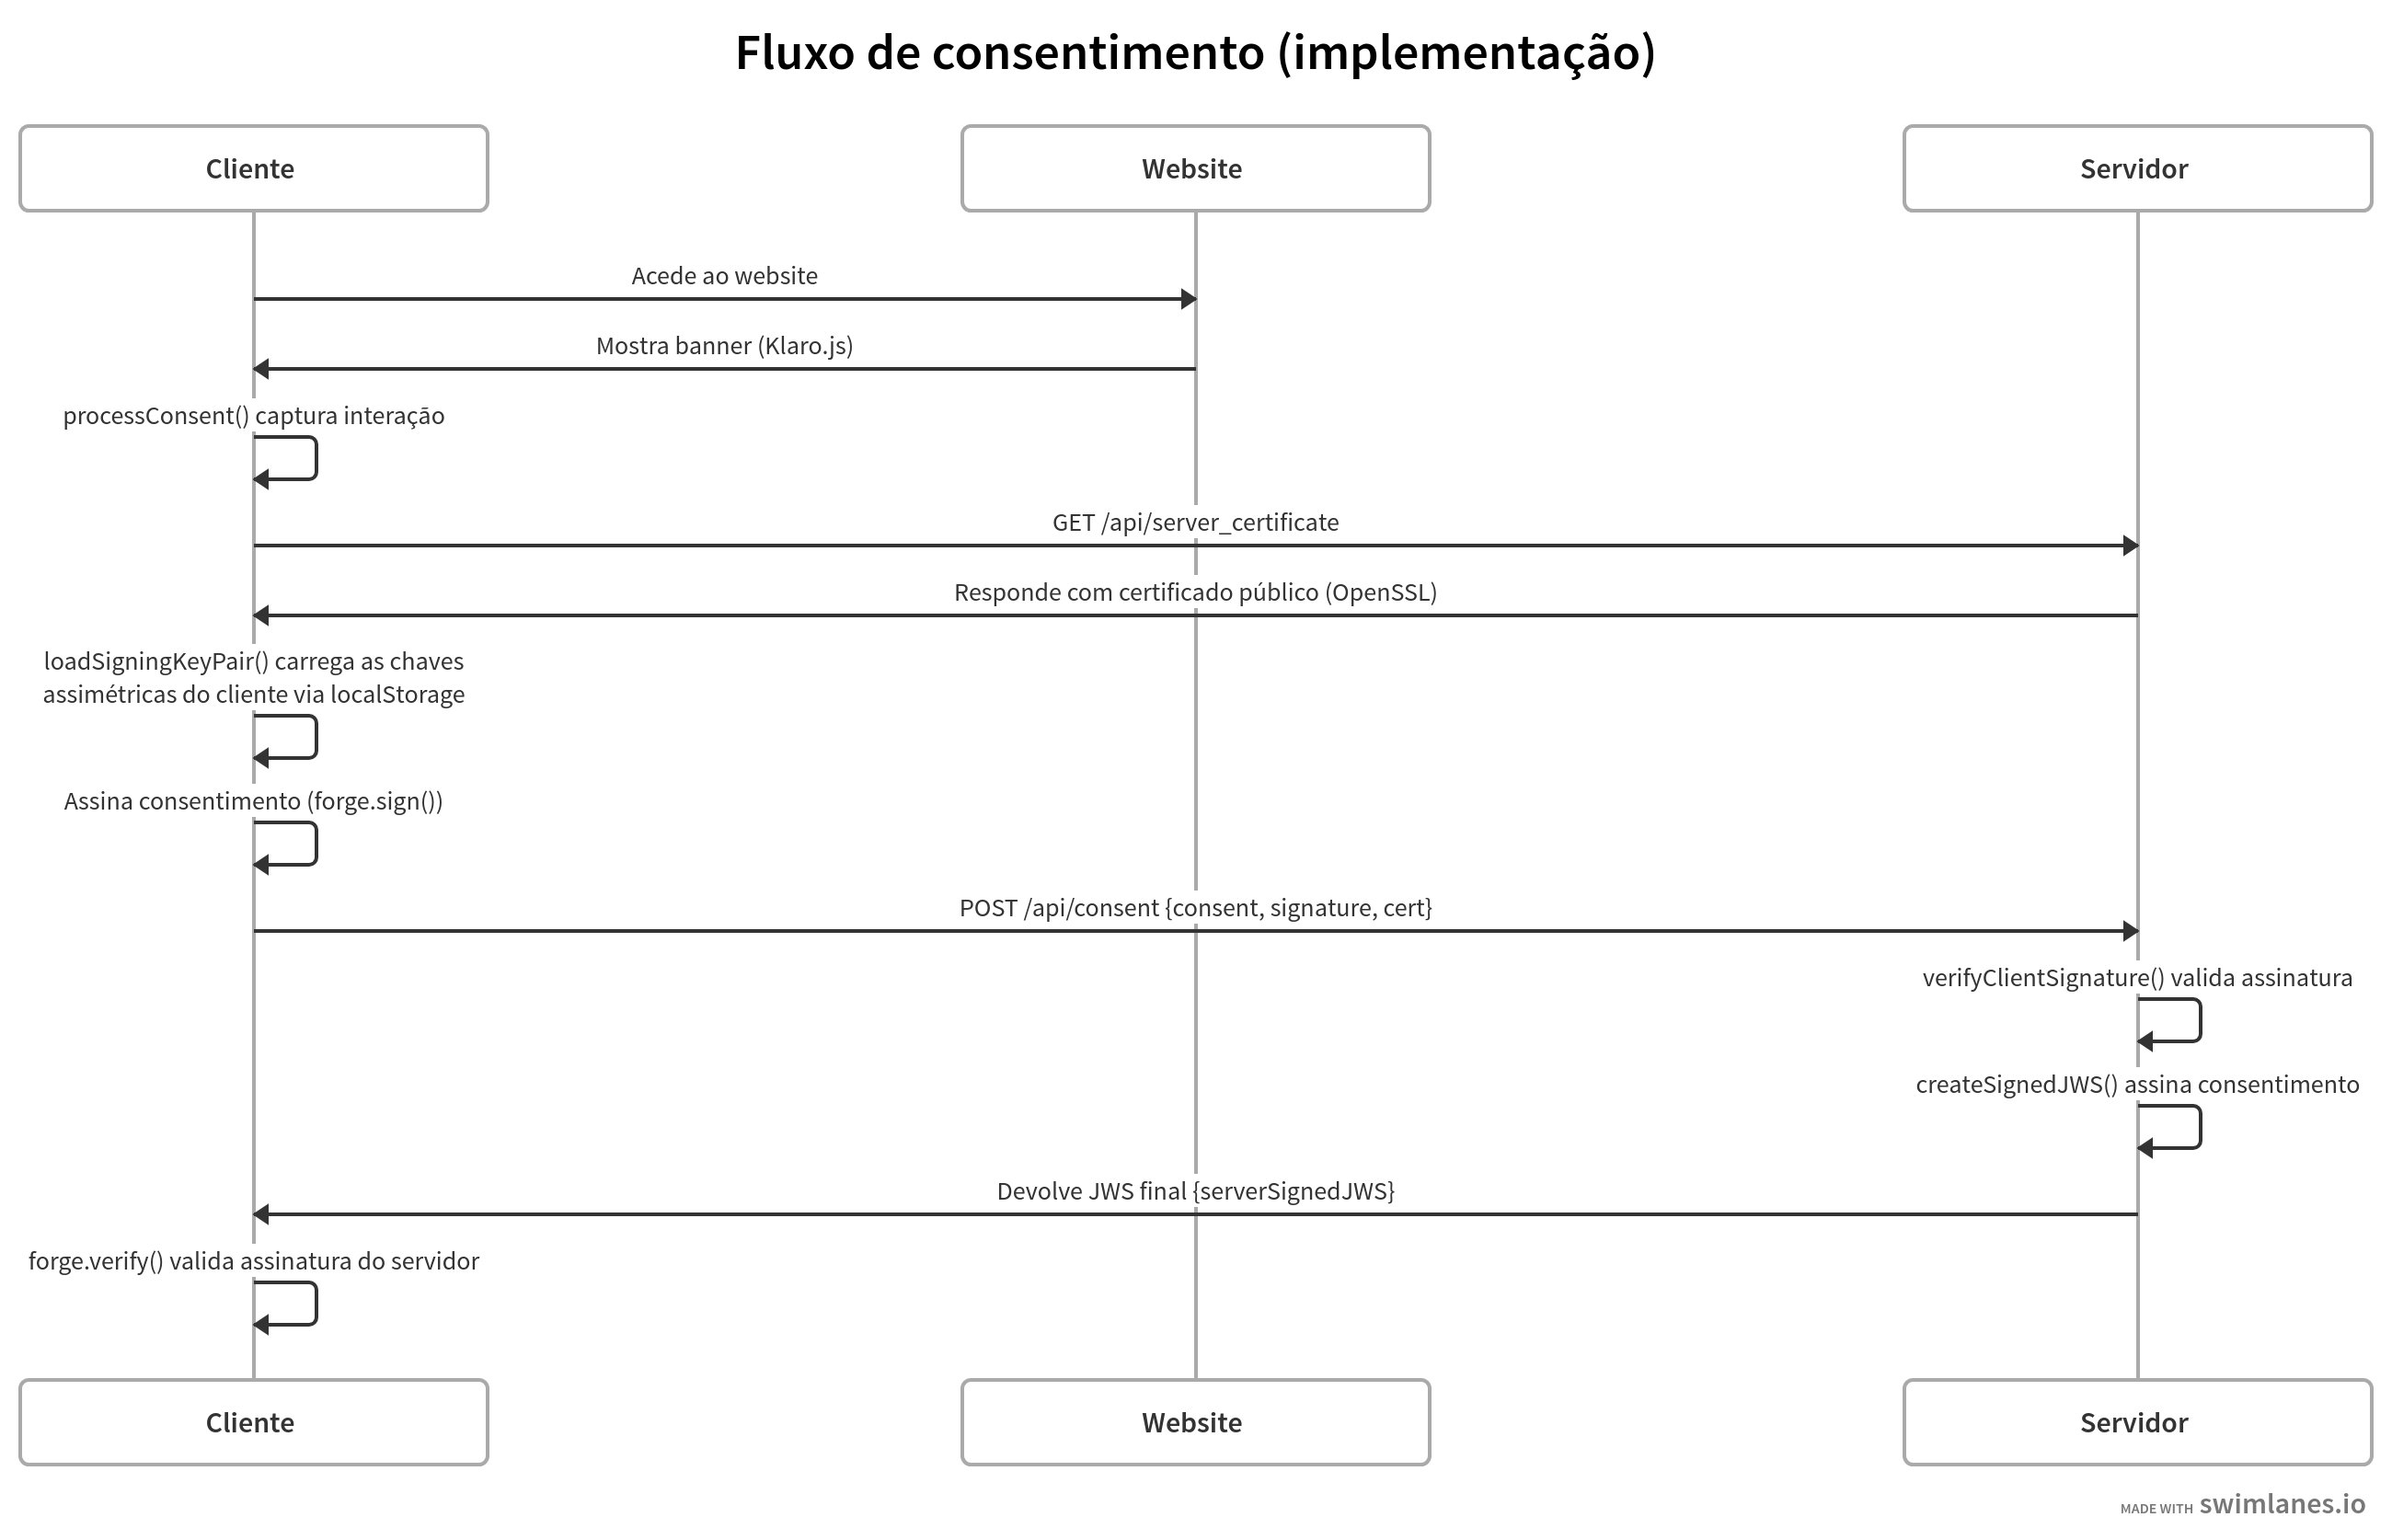
\includegraphics[width=1\textwidth]{images/swimlanes_solution.png}
\end{center}
\caption{Diagrama do protocolo.}
\label{fig:swimlane-solution}
\end{figure}

\newpage

\subsection{Registo do consentimento}

O registo do consentimento, juntamente com as respetivas assinaturas, constitui o resultado final do fluxo implementado. Trata-se de um registo digital que comprova a aceitação ou rejeição, pelo utilizador, de determinados serviços ou finalidades. Este registo é implementado sob a forma de um \textit{JSON Web Signature} (\textit{JWS}), que encapsula o \textit{payload} com os detalhes do consentimento do utilizador, a assinatura digital do cliente — garantindo que foi efetivamente o utilizador a autorizar — e a assinatura digital do servidor, que confirma a validação e integridade do consentimento.

O \textit{JWS} é mantido por ambas as entidades, cliente e servidor, permitindo consultas futuras, auditoria e eventual revogação do consentimento. Este mecanismo assegura a \textit{autenticidade}, uma vez que a assinatura do cliente comprova que o consentimento foi emitido pela pessoa correta; a \textit{integridade}, já que qualquer alteração no \textit{payload} invalida as assinaturas e impede a manipulação; e o \textit{não repúdio}, pois o cliente não pode negar a sua decisão devido à assinatura digital inequívoca, nem o servidor pode negar que conhece a decisão do utilizador.

Podemos consultar no apêndice \ref{apendice:jws-client} a implementação do \textit{JWS} do lado do cliente.

O \textit{JWS} resultante contém dois elementos principais:

\begin{itemize}
    \item \textit{Payload}: o \textit{payload} codificado em \textit{base64} com os dados do consentimento do utilizador.
    \item \textit{Signatures}: um array com uma ou mais assinaturas digitais. Neste caso, inclui a assinatura do cliente e a assinatura do servidor.
\end{itemize}

Um exemplo de \textit{JWS} gerado é o seguinte:

\begin{lstlisting}
{
  "payload": "eyJjb25zZW50cyI6eyJ0d2l0dGVyIjpmYWxzZSw ...",
  "signatures": [
    {
      "header": {"typ": "JWT", "alg": "PS256"},
      "signature": "b1Xn5AaxYZWZNfHoeL-SWTAySbT8yFWjJiPTK_rlIoPwTdukp9wpn..."
    },
    {
      "header": {"typ": "JWT", "alg": "PS256"},
      "signature": "BPVz73atRIFhzRx6YVsHWOkEX6Rb-hL0XoahOc2uxX9EPDs5RSVvYuNzpoX_Vv..."
    }
  ]
}
\end{lstlisting}

Esta estrutura assegura que tanto o cliente como o servidor possuem uma prova verificável do consentimento, permitindo auditoria, revogação ou consulta futura. Deste modo, o mecanismo implementado cumpre os objetivos definidos na criação desta prova de conceito, pois fornece uma forma de registar e gerir consentimentos de forma transparente e técnica, garantindo a criação de registos verificáveis, imutáveis e não repudiáveis.

A solução permite não só a recolha e gestão dos consentimentos dos utilizadores, mas também possibilita auditar os consentimentos em caso de não cumprimento, promovendo a transparência e fornecendo evidência técnica irrefutável de que as decisões dos utilizadores foram, ou não foram, respeitadas no tratamento dos dados. Embora não garanta a conformidade integral dos prestadores de serviços com regulamentos como o \acrshort{rgpd}, o sistema permite aos utilizadores demonstrar a não-conformidade em caso de violação das suas escolhas de privacidade, cumprindo assim os objetivos principais do projeto. Os testes funcionais e de desempenho descritos no Capítulo~\ref{cap:avaliacao} confirmam a viabilidade do modelo, validando o fluxo de consentimento, a criação e verificação de \textit{JWS} e a robustez das assinaturas digitais.

\section{Síntese do capítulo}

Neste capítulo foram apresentadas duas fases complementares da implementação da solução proposta. A prova de conceito permitiu validar a arquitetura conceptual, demonstrando a viabilidade técnica dos princípios de integridade, autenticidade, não repúdio, transparência e auditabilidade num modelo simplificado. Seguiu-se o desenvolvimento da prova de conceito, integrando cliente, servidor e interface web, com a utilização de certificados digitais, assinaturas e o formato \textit{JWS} para criar registos de consentimento auditáveis e verificáveis. Foram realizados testes funcionais e de desempenho, descritos no Capítulo~\ref{cap:avaliacao}, que confirmaram o correto funcionamento do fluxo de consentimento e a robustez das assinaturas digitais.  

No capítulo seguinte é apresentada a avaliação da implementação, abordando tanto os aspetos funcionais como de desempenho. Serão analisados os testes realizados e os resultados obtidos, de forma a demonstrar a fiabilidade, robustez e eficiência da arquitetura desenvolvida, evidenciando o cumprimento dos objetivos definidos neste trabalho.
